%%%%%%%%%%%%%%%%%%%%%%%%%%%%%%%%%%%%%%

\documentclass[12pt]{article}
%\documentstyle[12pt,psfig,epsf]{article}

\hoffset=-15mm \voffset=-25mm \textwidth=165mm \textheight=245mm
\usepackage{graphicx}
\usepackage{amsmath}
\usepackage{amssymb}
%\usepackage{bigcircle}
\usepackage{wrapfig}
\usepackage{indentfirst}
\usepackage{color}
\usepackage{subfigure}

\begin{document}

\vskip 0.5cm \centerline{\bf\Large Vector meson production}
\centerline{\bf\Large in ultra-peripheral collisions at hadronic colliders}  \vskip 0.3cm
\centerline{R.~Fiore $^a$, L.~Jenkovszky $^{b\star}$, V.~Libov$^{c\diamond}$, and Magno V. T. Machado$^d$}

\vskip 1cm

\centerline{$^a$ \sl Universita' della Calabria}
\centerline{$^b$ \sl Bogolyubov Institute for Theoretical Physics,
National Academy of Sciences of Ukraine} \centerline{\sl Kiev,
03680 Ukraine}
\centerline{$^c$ \sl Deutsches Elektronen-Synchrotron, Hamburg, Germany}
\centerline{$^d$ \sl HEP Phenomenology Group, CEP 91501-970, Porto Alegre, RS, Brazil
}
\vskip
0.1cm

\begin{abstract}\noindent
By using a Regge-pole model for vector meson production (VMP), successfully describing the HERA data, we analyse the correlation between VMP cross sections in photon-induced reactions at HERA and those in ultra-peripheral collisions at the LHC.
Predictions for future experiments on production of $J/\psi$ and other vector mesons are presented.
\end{abstract}

\vskip 0.1cm

$
\begin{array}{ll}

^{\star}\mbox{{\it e-mail address:}} &
   \mbox{jenk@bitp.kiev.ua} \\
^{\diamond}\mbox{{\it e-mail address:}} &
   \mbox{vladyslav.libov@desy.de} \\

\end{array}
$

%\end{titlepage}

\section{Introduction}\label{Int}

After the shutdown of HERA, exclusive diffractive production of mesons in ultra-peripheral collisions of protons and nuclei became among the priorities of the present and future studies at the LHC \cite{LHCb1, LHCb2}, triggering a large number of theoretical investigations \cite{Schafer, Brazil, Ryskin, Motyka, Szczurek, Recent}.
For relevant review papers see, e.g. \cite{Review}.
First results on vector meson production, in particular of $J/\psi$, are already published \cite{LHCb1, LHCb2}.

In this study of vector meson production at the LHC we scrutinize possible changes in the energy dependence of the cross sections when moving from HERA to the LHC, in particular we are interested in the change from "soft" (light vector mesons) to those heavy ($\phi,\ \ J/\psi,\ \ \Upsilon$ {\it etc.}) mesons;

\section{VMP at HERA}
At HERA, VMP was studied in details both by the H1 and ZEUS collaborations. Most of the events were chosen in the 
kinematical region corresponing to diffractive scattering, which means that the processes can be described by a Pomeron exchange, see Fig. \ref{fig:diagrams}. Pomeron dominance is especially clean in $J/\Psi$ production, where,
by the Zweig (OZI) rule, any exchange of secondary trajectories made of quarks is forbidden, leaving and uncontaminated Pomeron exchange alone.  This does not mean that the dynamics is simple, but we have the opportunity 
to scrutinize in this class of reactions the nature of the Pomeron, a complicated and controversial object. 
The main problem is the twin nature of the Pomeron: it seems to be "soft" or "hard" depending on the virtuality of the incident photon and/or mass of the produced vector meson.   
     
\begin{figure}[!h]
\centering
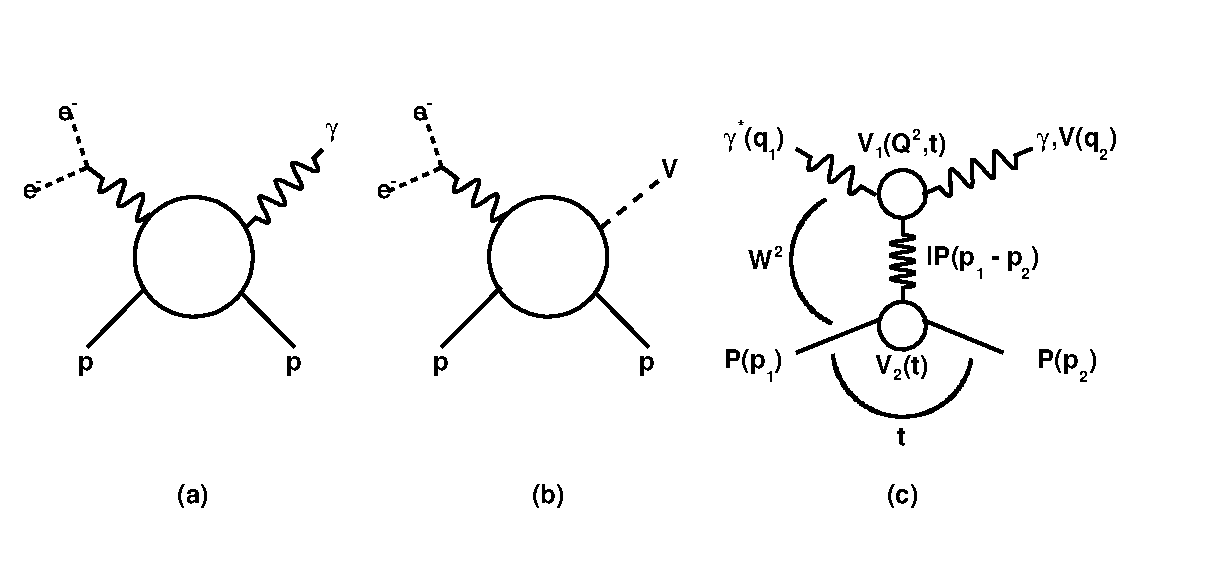
\includegraphics[width=.8\textwidth]{figures/diagrams.eps}
\caption{Diagrams of DVCS (a) and VMP (b); (c) DVCS (VMP) amplitude in a Regge-factorized form.}
\label{fig:diagrams}
\end{figure}

In most of the papers on the subject the existence of two Pomerons is assumed: a hard or QCD pomeron, resulting
from perturbative quantum chromodynamic calculations, and a soft, somewhat misleadingly called "non-perturbative". 
Instead, we believe that there is only one Pomeron in Nature, but it has two components, whose relative weight is 
regulated by relevant $\tilde Q^2$-dependent factors in front of the two, where the measure of the "hardness" $\tilde Q^2=Q^2+M_V^2$ is the sum of the squared photon virtuality and the produced vector meson's mass.  

A specific model realizing this idea was constructed and tested against the experimental data recently (see
Ref.~\cite{FFJS} and earlier references therein). The relevant VMP amplitude reads 
  $$
   A(s,t,Q^2,{M_v}^2)= \widetilde{A_s}e^{-i\frac{\pi}{2}\alpha_s(t)}\left(\frac{s}{s_{0}}\right)^{\alpha_s(t)}
    e^{b_st - n_s\ln{\left(1+\frac{\widetilde{Q^2}}{\widetilde{Q_s^2}}\right)}}
  $$
  \begin{equation}
  +\widetilde{A_h}e^{-i\frac{\pi}{2}\alpha_h(t)}\left(\frac{s}{s_{0}}\right)^{\alpha_h(t)}
    e^{b_ht - (n_h+1)\ln{\left(1+\frac{\widetilde{Q^2}}{\widetilde{Q_h^2}}\right)}
    +\ln{\left(\frac{\widetilde{Q^2}}{\widetilde{Q_h^2}}\right)} },
    \label{eq:Amplitude_FFJS}
    \end{equation}
 where  $\alpha_s(t)$ and and $\alpha_h(t)$ are the soft and hard Pomeron trajectories. Let us 
stress that the Pomeron is unique in all reactions, just its components (and perameters) change from one reaction
to another. Examples with detailed fits can be found in recent papers \cite{FFJS}.

The integrated (also called total) cross VMP cross section can be simply calculated without integration for an exponential diffraction cone according to the formula
$$\sigma_{el}(s)=\frac{1}{B(s)}\frac{d\sigma}{dt}\biggr\rvert_{t=0.}$$ 

Since our primary goal is the comparison between the energy dependence of VMP at HERA and the LHC, we start with a very simple ansatz for the $\gamma p\rightarrow Vp$ cross section, postponing the use of the advanced model  
Eq. (\ref{eq:Amplitude_FFJS}) to a future study.

\section{VMP at the LHC} 
%\section{Simple parametrizations of $\sigma_{\gamma p\rightarrow Vp}(\omega)$;\\
%The photon flux}\label{simple}

Vector meson production (VMP) cross section, Fig. 1, can be written in a factorized form, see \cite{Brazil, Review} (e.g. Eqs. (1) and (9) in \cite{Brazil}a)).
The distribution in rapidity $Y$ of the production of a vector meson $V$ in the reaction $h_1+h_2\rightarrow h_1Vh_2,$ (where $h$ may be a hadron, e.g. proton, or a nucleus, pPb, PbPb,...) is calculated according to a standard prescripion based on the factorization of the photon flux and photon-proton cross section (see below).

\begin{figure}[!h]
\centering
 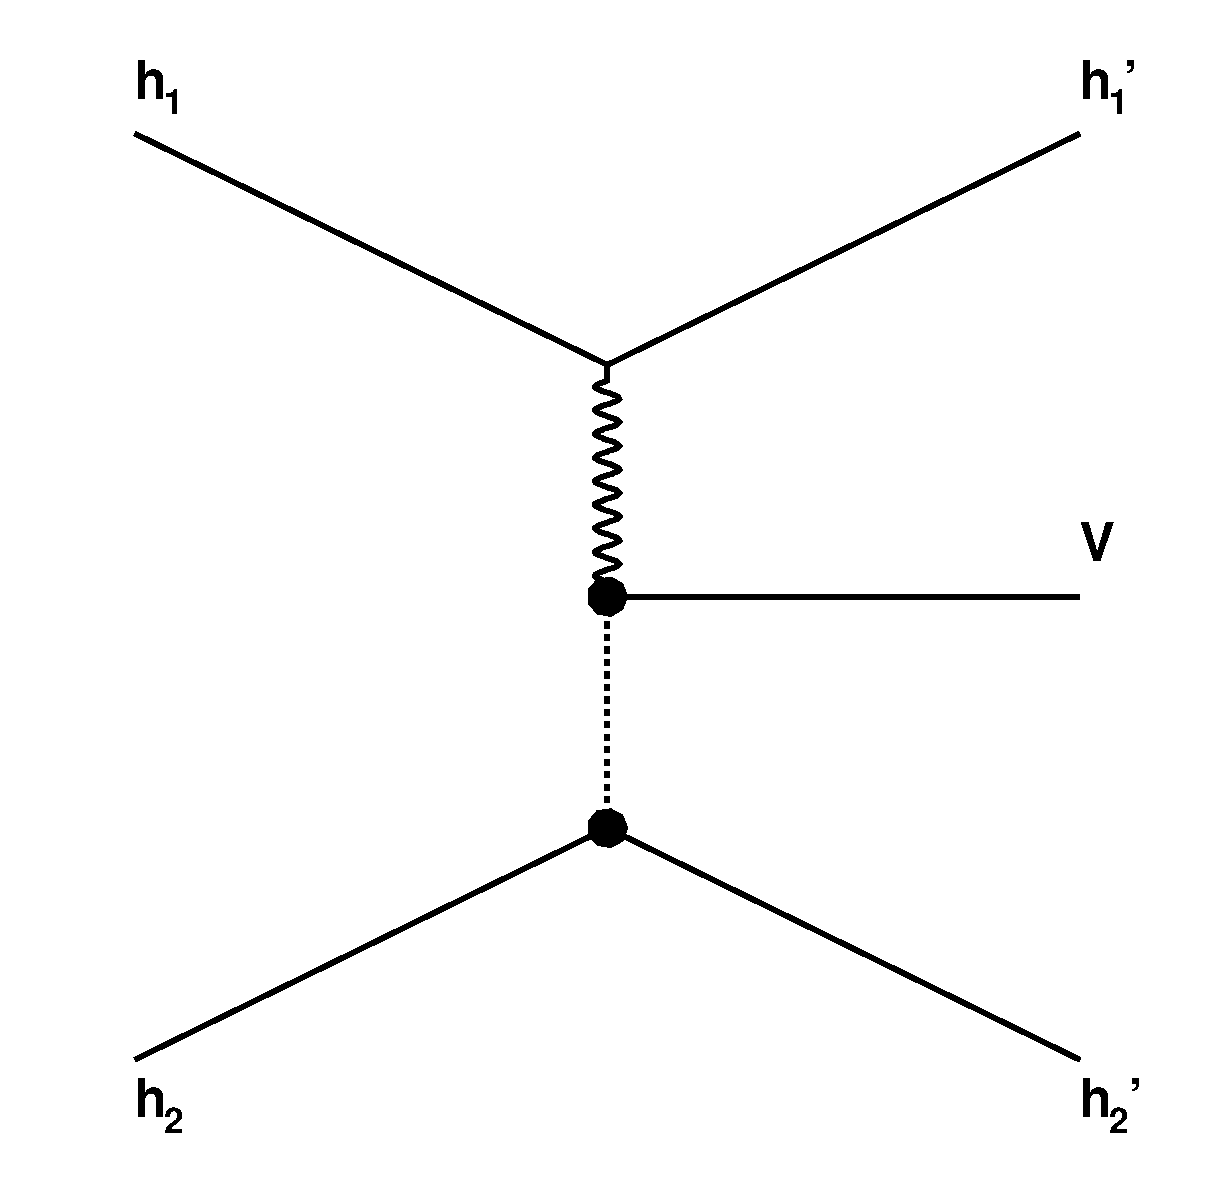
\includegraphics[width=.4\textwidth]{figures/exclusive_vmp.eps}
 \caption{Feynman diagram of vector meson production in hadronic collision.}
 \label{fig:vmp_feynman}
\end{figure}

Generally speaking, the $\gamma p$ cross section depends on three variables: the total energy of the $\gamma p$ system, $W$,
the squared momentum transfer at the proton vertex, $t$, and virtuality $\tilde Q^2=Q^2+M_V^2$, where $Q^2=-q^2$ is the photon virtuality. Since, by definition, in ultraperipheral, $b>>R_1+R_2,$
collisions, where $b$ is the impact parameter, i.e. the closest distance between the centres of the colliding particles/nuclei and R is their radii,
photons are nearly real, $Q^2=0$, and $M_V^2$ remains the only measure of "hardness" (NB: this might not be true for the peripheral $b\sim R_1+R_2$ collisions and in
Pomeron or Odderon exchange instead of the photon). Finally, the $t$-dependence (shape of the diffraction cone) is known to be nearly exponential. It can be either integrated, or
kept explicit. Extending this parametrization to include a $t-$dependent exponential is easy (see below).
In any case, $\sigma_{\gamma p\rightarrow Vp}(\tilde Q^2, t, W)$, is well known from HERA.

To start with, we use VMP cross sections integrated in $t$ equivalently, the relevant differential cross section
at $t=0$ divided by its foward slope $B$.

%{\tiny\bf (I added  $Q^2$, $t$ as arguments since at this point we haven't yet said explicitely that we consider $t$ %integration.)}

To start with, we use a simple parametrization of the $\sigma_{\gamma p\rightarrow Vp}(W)$ cross section, $\sigma_{\gamma p\rightarrow Vp}(W)=\int_{t_m}^{t_{thr}}\frac{d\sigma}{dt},$
suggested by Donnachie and Landshoff \cite{DL}: $\sigma(W)\sim W^{\delta},\ \delta\approx 0.8$ (more involved models, e.g. of Ref. \cite{Capua, Fazio} will be considered below).

The differential cross section as a function of rapidity reads:
 \begin{equation}\label{1}
\frac{d\sigma (h_1+h_2\rightarrow h_1+V+h_2)}{dY}=\omega_+\frac{dN_{\gamma/h_1}(\omega_+)}{d\omega}\sigma_{\gamma h_2\rightarrow Vh_2}(\omega_+)+
\omega_-\frac{dN_{\gamma/h_2}(\omega_-)}{d\omega}\sigma_{\gamma h_1\rightarrow Vh_1}(\omega_-),
\end{equation}
where $\frac{dN_{\gamma/h}(\omega)}{d\omega}$ is the "equivalent" photon flux \cite{Review}
$\frac{dN_{\gamma/h}(\omega)}{d\omega}=\frac{\alpha_{em}}{2\pi\omega}[1+(1-\frac{2\omega}{\sqrt{s}})^2]
(\ln\Omega-\frac{11}{6}+\frac{3}{\Omega}-\frac{3}{2\Omega^2}+\frac{1}{3\Omega^3})$
and $\sigma_{\gamma p\rightarrow Vp}(\omega)$ is the total (integrated over $t$) cross section of the vector meson photoproduction subprocess (same as e.g. at HERA, see \cite{Capua, Fazio}). Here $\omega$ is the photon energy, $\omega=W^2_{\gamma p}/2\sqrt s_{pp}$ with
$\omega_{min}=M_V^2/(4\gamma_Lm_p),$ where $\gamma_L=\sqrt s/(2m_p)$
is the Lorentz factor (Lorentz boost of a single beam), e.g., for pp at the LHC for $\sqrt{s}=7$~TeV,
$\gamma_L=3731$.
%,giving $W_{\gamma p}=960$ GeV.
Furthermore,
$\Omega=1+Q_0^2/Q_{min}^2,\  Q_{min}^2=\omega/\gamma_L^2,\   Q_0^2=0.71GeV^2,\   x=M_Ve^{(-y)}/\sqrt s,\  Y\sim\ln(2\omega/m_V)$ is rapidity, $y=Y(?$).
Furthermore we have: $\Omega=1+Q^2_0/Q^2_{min}$, where $Q_0^2=0.71,\ \ Q_{min}^2=\omega/\gamma^2_L,\ \omega=m_Ve^Y/2$, hence $\Omega_i=1+0.71\gamma_L^2,\ \ \gamma_L^2=7/(2m_p)\approx 3.57, \  \
m_{V=J/\psi}=3.1, \sqrt{s}=7, \ \alpha_{em}/(2\pi)\approx 10^{-3},$ hence $Q^2_{min}\approx 5.54e^Y,\ \ \Omega=1+3.9e^{-Y}$. For definiteness we fix: a) the colliding particles are protons;
b) the produced vector meson $V$ is $J/\psi$, and 3) the collision energy $\sqrt s=7$ TeV.
We comprise the constants in $A=\alpha_{em}/(2\pi),\ \  c=Q_0^2\gamma_L^2$.
(Note that the shape of the distribution in $Y$ is very sensitive to the value and the sign of the constant $c$).
The $i=\pm$ signs of $\omega$ correspond to the first or second term in Eq. (\ref{1}), respectively, $\omega_{\pm}\sim e^{\pm Y}$.

\subsection{Corrections for rapidity gap survival probabilities}\label{corrections}
The above results may be modified by initial and final state interactions,
alternatively called as rescattering corrections. Calculation of these
corrections is by far not unambiguous, the result depending both on the input
and on the unitarization procedure chosen. The better (more realistic) the input, the smaller the unitarity (rapidity gap survival probability) corrections.
Since this is a complicated and controversial issue {\it per se} deserving special studies beyond the scope of the present paper, to be coherent with the "common trend", here we use only familiar results from the literature:
the standard prescription is to multiply the scattering amplitude (cross section) by a factor (smaller than one), depending on energy and eventually other kinematical variables~\cite{Ryskin}.
In this work we used a constant value of 0.8.

\section{Results}

In this section, theoretical predictions are presented and compared to data.
Calculations use two models for the exclusive $J/\Psi$ photoproduction cross section, $\sigma_{\gamma p \to J/\Psi}$:
the simple power-law, $\sigma_{\gamma p \to J/\Psi}\sim W^\delta$, with $\delta=0.8$, and the so-called geometric model.
The latter model was suggested and applied to deeply virtual Compton scattering (DVCS) in Ref.~\cite{Capua}.
Apart from $W$ and $t$, it contains alwo dependence on virtuality $Q^2$.
The model was fitted to the HERA data on DVCS, but it can be applied also to vector meson production (VMP) by refitting its parameters.
Instead, below we shall use two versions of the so-called Reggeometric model of VMP and DVCS, suggested in Refs. \cite{Fazio}a) and \cite{Fazio}b).
Its first version \cite{Fazio} a) applies to photoproduction ($Q^2=0$), and the integrated photoproduction cross section, Eq. (11) in Ref. \cite{Fazio}a), is
\begin{equation}
\sigma_{\gamma p \to J/\Psi}=A_0^2\frac{(W/W_0)^{4(\alpha_0-1)}}{(1+\tilde Q^2/Q^2_0)^{2n}[4\alpha'\ln(W/W_0)+4\Bigl(\frac{a}{\tilde Q^2}+\frac{b}{2m_N^2}\Bigr)]},
\end{equation}
where $\tilde Q^2=Q^2+m_V^2$ and the parameters, fitted \cite{Fazio}a) to $J/\psi$ photoproduction, quoted in
Table II of Ref. \cite{Fazio}a), are: $A_0=29.8\pm 2.8,\ \ Q_0^2=2.1\pm 0.4,\ \
n=1.37\pm 0.14,\ \ \alpha_0 =1.20\pm 0.02,\ \ \alpha'=0.17\pm 0.05, a=1.01\pm 0.11,\ \ b=0.44\pm 0.08,\ \ W_0=1$ and relevant dimensions here again are implied.
Note that compared to the original formula, $s$ was replaced by $W^2$, since $W$ is used in this paper to 
denote the photon-proton centre-of-mass energy (in contrast, $\sqrt{s}$ in this paper is the proton-proton centre-of-mass energy).

Figure~\ref{fig:dSigma_dy_nodata} shows the predicted cross sections of $J/\Psi$ production at LHC ($\sqrt{s}=7$ TeV) as a function distribution in rapidity $Y$.
Generally, the power law and geometric model yield similar distributions,  the latter is flatter though.
Figure~\ref{fig:dSigma_dW_nodata} shows the $W$-dependence of $J/\psi$ photoproduction cross section.
Again, two models are generally similar.
\newpage

\begin{figure}[!t]
  \centering
  \subfigure[]{\label{fig:dSigma_dy_nodata}
    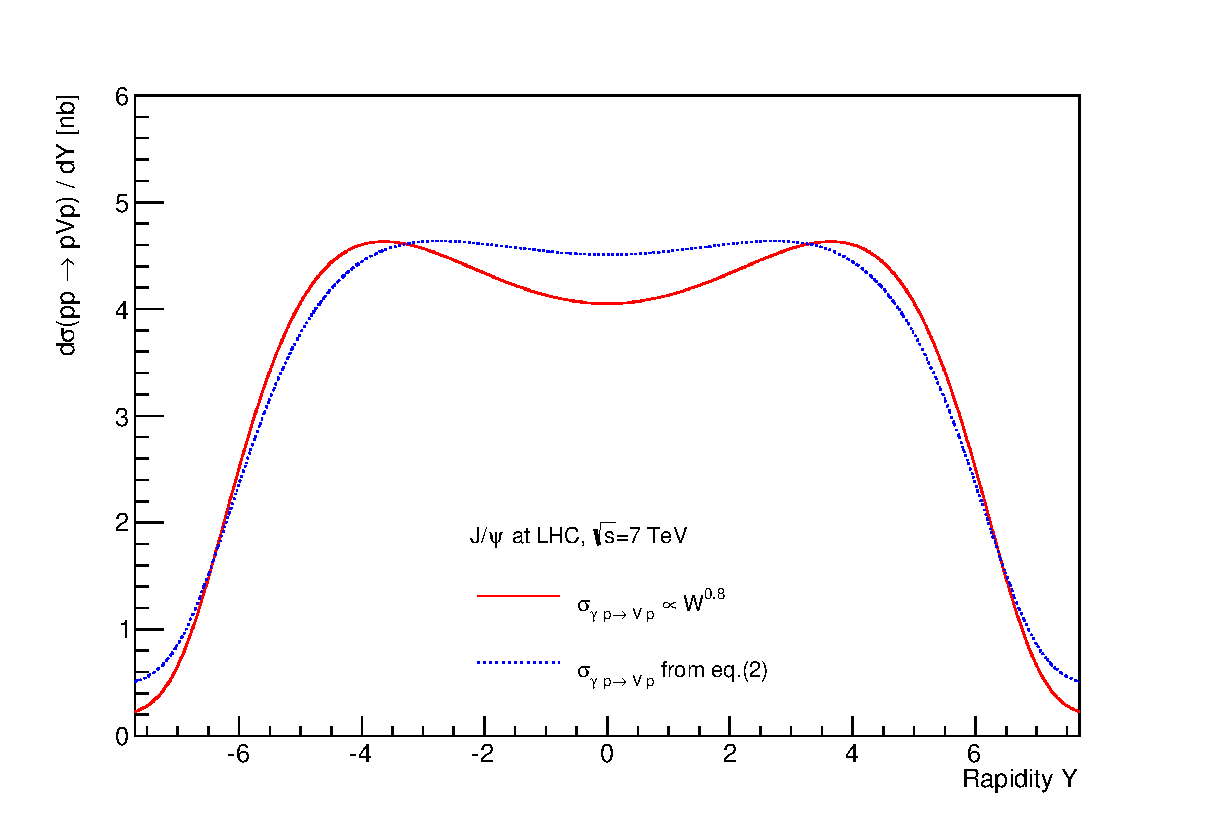
\includegraphics[height=6.5cm,width=0.46\textwidth]{figures/dSigma_dy_nodata.eps}
  }
  \subfigure[]{\label{fig:dSigma_dW_nodata}
    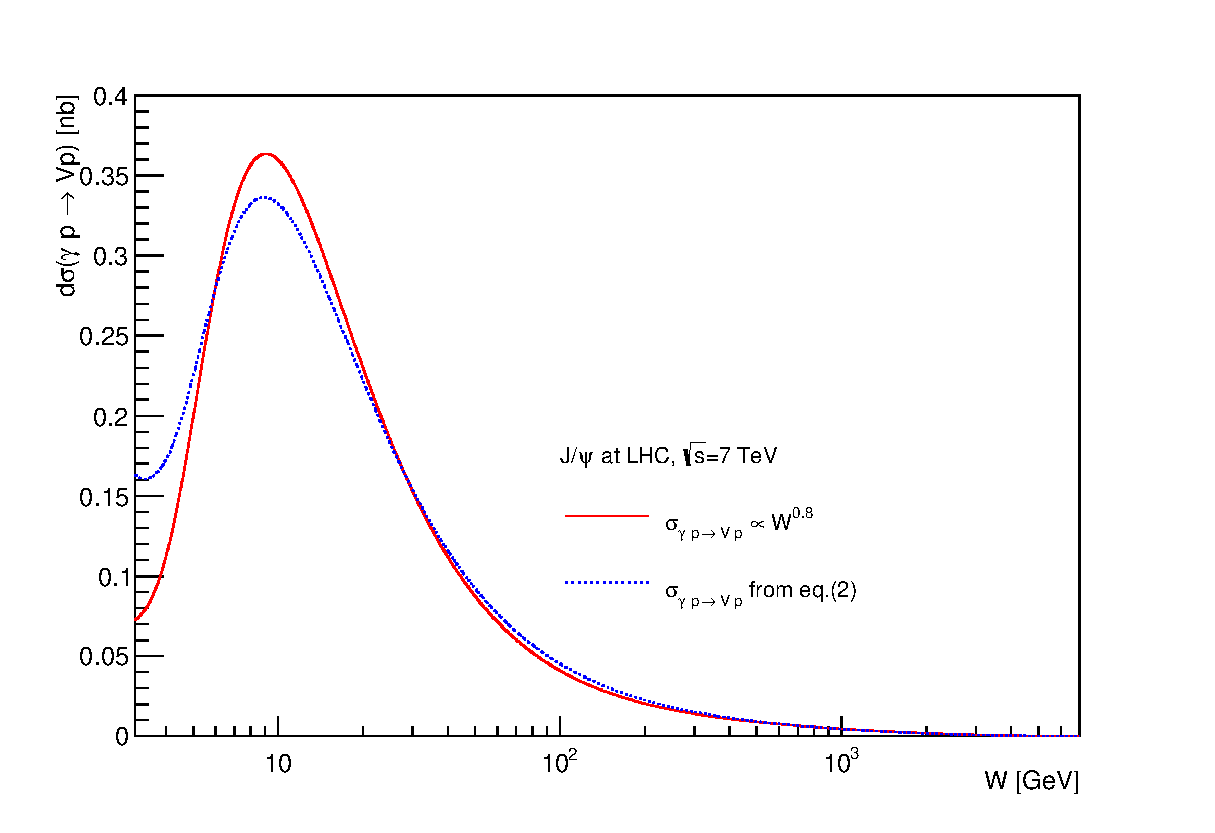
\includegraphics[height=6.5cm,width=0.46\textwidth]{figures/dSigma_dW_nodata.eps}
  }
  \caption{Differential cross section of exclusive $J/\psi$ production at LHC as a function of rapidity $Y$ (a) and of the photon-proton centre-of-mass energy $W$ (b).
           The red curves represent the simple power-law parameterisation of the photon-proton cross section, while the blue curves use the geometric model.}
\end{figure}

The LHCb~\cite{LHCb1, LHCb2} experiment at LHC has recently measured production cross section of $J/\Psi$ as a function of rapidity.
Fig.~\ref{fig:dSigma_dy_comparison1} shows a comparison of our calculations to these data.
As can be seen, data are somewhat steeper than both of the curves.
LHCb also extracted the basic photon-proton photoproduction cross section as a function of $W$ from their rapidity data.
The result is compared to our predictions in  Fig.~\ref{fig:sigma_gamma_p_W_powerlaw_vs_geometric}.
Also ZEUS and H1 data are shown.

\begin{figure}[!h]
  \centering
  \subfigure[]{\label{fig:dSigma_dy_comparison1}
    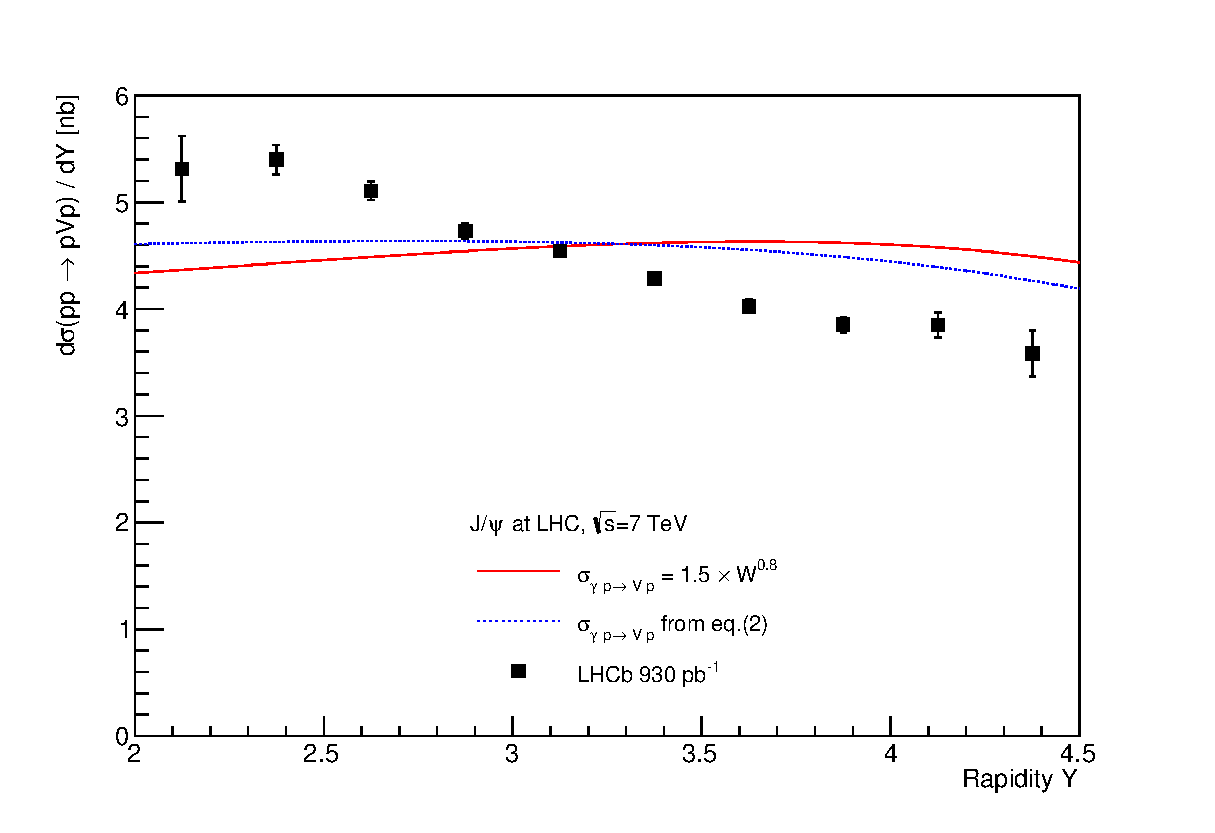
\includegraphics[height=6.5cm,width=0.46\textwidth]{figures/dSigma_dy_comparison1.eps}
  }
  \subfigure[]{\label{fig:sigma_gamma_p_W_powerlaw_vs_geometric}
    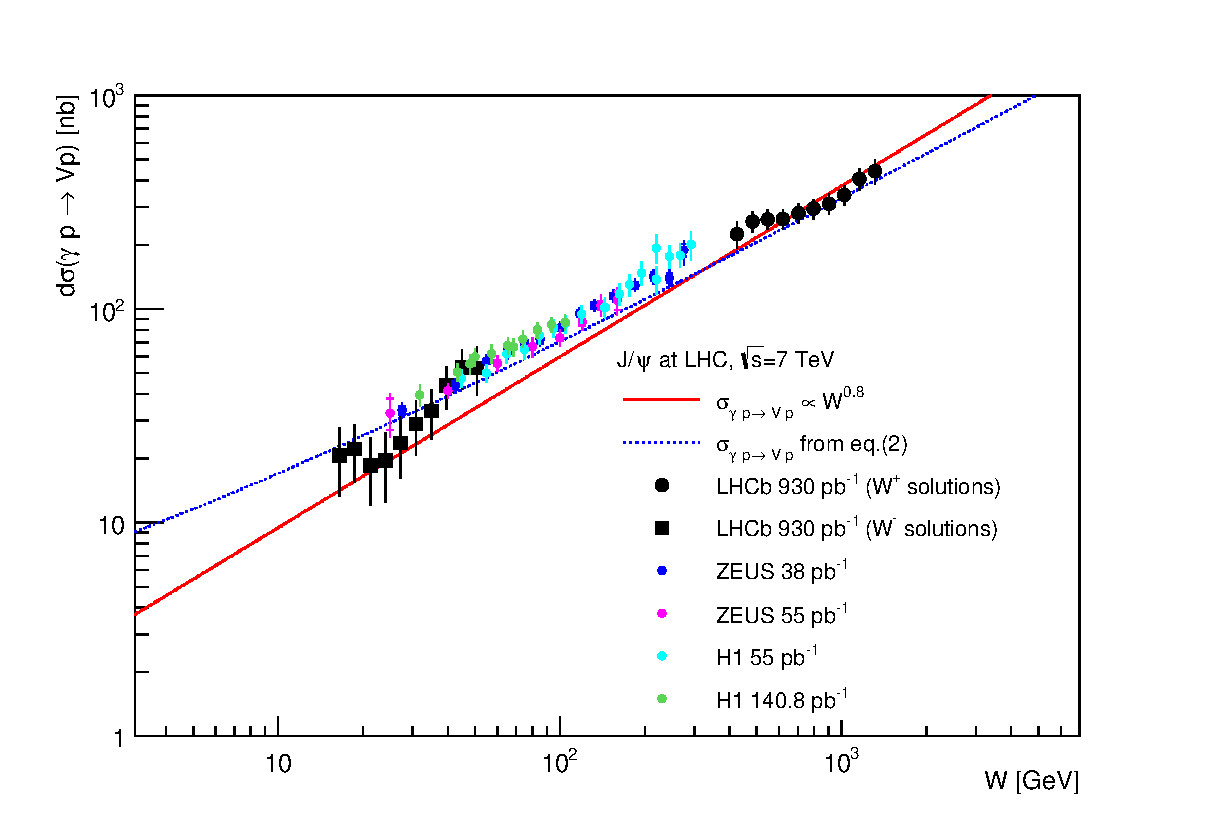
\includegraphics[height=6.5cm,width=0.46\textwidth]{figures/sigma_gamma_p_W_powerlaw_vs_geometric.eps}
  }
  \caption{Differential cross section of $J/\psi$ production at LHC as a function of rapidity $Y$ together with LHCb data (a). $J/\psi$ photoproduction ($\gamma p \to J/\psi p$) cross section as a function photon-proton centre-of-mass energy compared
           with LHCb, ZEUS and H1 data (b).}
\end{figure}

\subsection{Fitting the power law to LHCb data}

As discussed above, LHCb rapidity data have a steeper shape than the predictions.
Here we investigate the role of the power $\delta$ in the rapidity cross section.
In particular, we perform a least-squares fit to these data.
The free parameters are the power $\delta$ and the overall normalization.
The best fit gives $\delta$=0.37 and is shown in Fig.~\ref{fig:delta_fit}.
Indeed, the prediction  obtained with this value gives a much better description of the rapidity distribution.
It is interesting  to compare to other parameterisations, in particular by using the
logarithimic parameterisation, which is less steep than than the power law.
This is shown  in Fig.~\ref{fig:all_curves}. The logarithm provides good description as well.
Figure~\ref{fig:dipole} shows, for completeness, predictions from other groups, together with LHCb rapidity data.
Good description of data is provided.

Our predictions are also compared to the H1 and ZEUS data~\ref{fig:all_curves_w}.
As can be seen, the geometric model provides the best description.
Power law with standard $\delta=0.8$ agrees reasonably as well.
However, the one with $\delta=0.37$, as well as the logarithm fail to describe the data.

\begin{figure}[!h]
\centering
 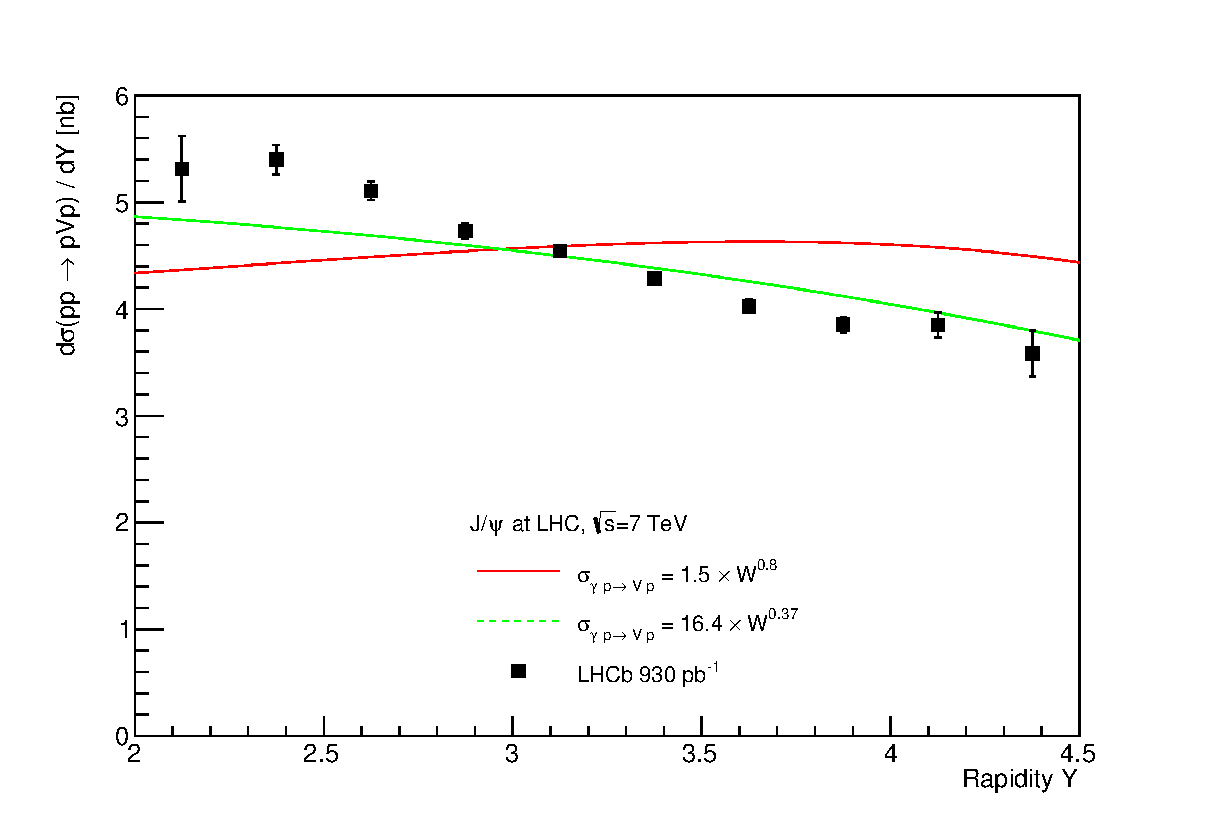
\includegraphics[width=.8\textwidth]{figures/dSigma_dy_comparison2.eps}
 \caption{Differential cross section of $J/\psi$ production at LHC as a function of rapidity $Y$ together with LHCb data.
          Both calculations use the simple power law model, with $\delta=0.8$ (red) and $\delta=0.37$ (green).
          See text for more details.}
 \label{fig:delta_fit}
\end{figure}

\begin{figure}[p]
\centering
 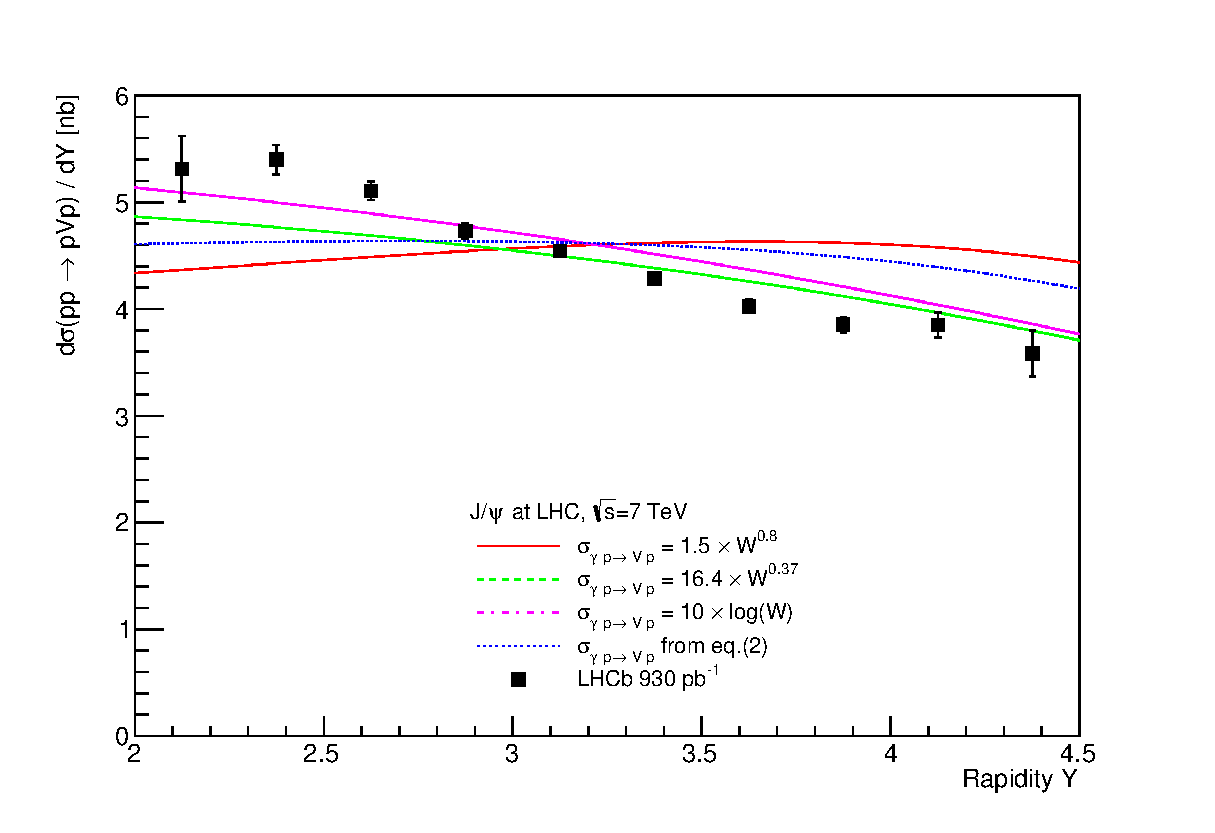
\includegraphics[width=.8\textwidth]{figures/dSigma_dy_comparison3.eps}
 \caption{Differential cross section of $J/\psi$ production at LHC as a function of rapidity $Y$ together with LHCb data.
          Various models for the photon-proton cross section were used: power law with $\delta=0.8$ and $\delta=0.37$ (red and green, respectively),
          logarithmic parameterisation (pink) and the geometric model (blue).
          }
  \label{fig:all_curves}
\end{figure}

\begin{figure}[p]
\centering
 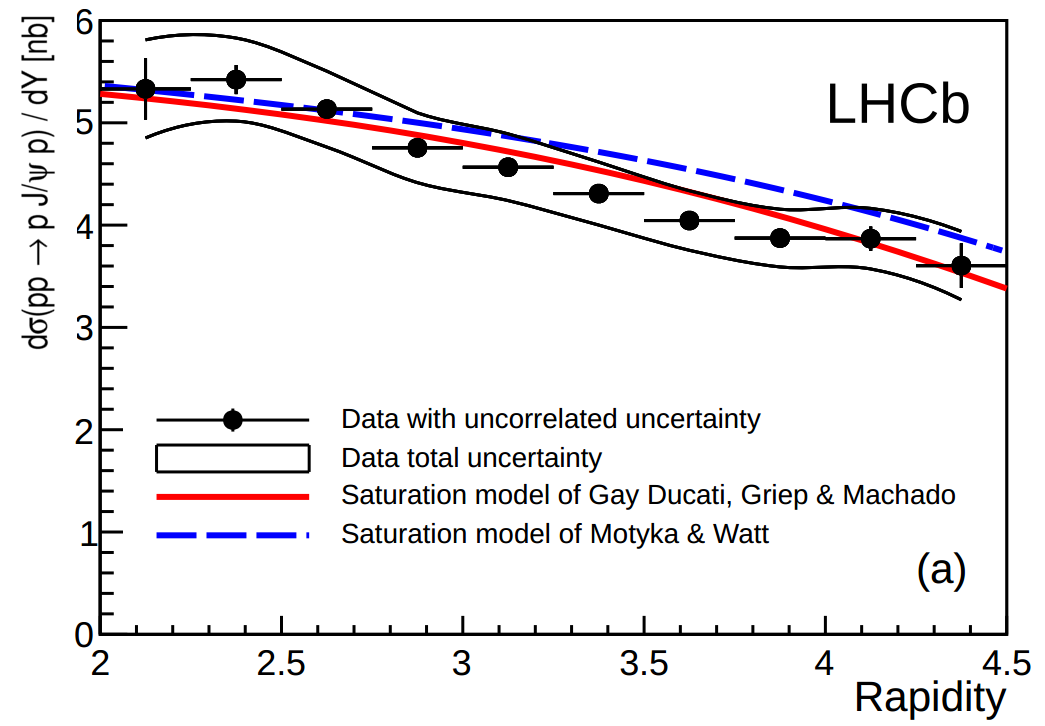
\includegraphics[width=.8\textwidth]{figures/Magno.png}
 \caption{Differential cross section of $J/\psi$ production at LHC as a function of rapidity $Y$ together with LHCb data.
         Taken from~\ref{LHCb2}.}
 \label{fig:dipole}
\end{figure}

\clearpage

\begin{figure}[!t]
\centering
 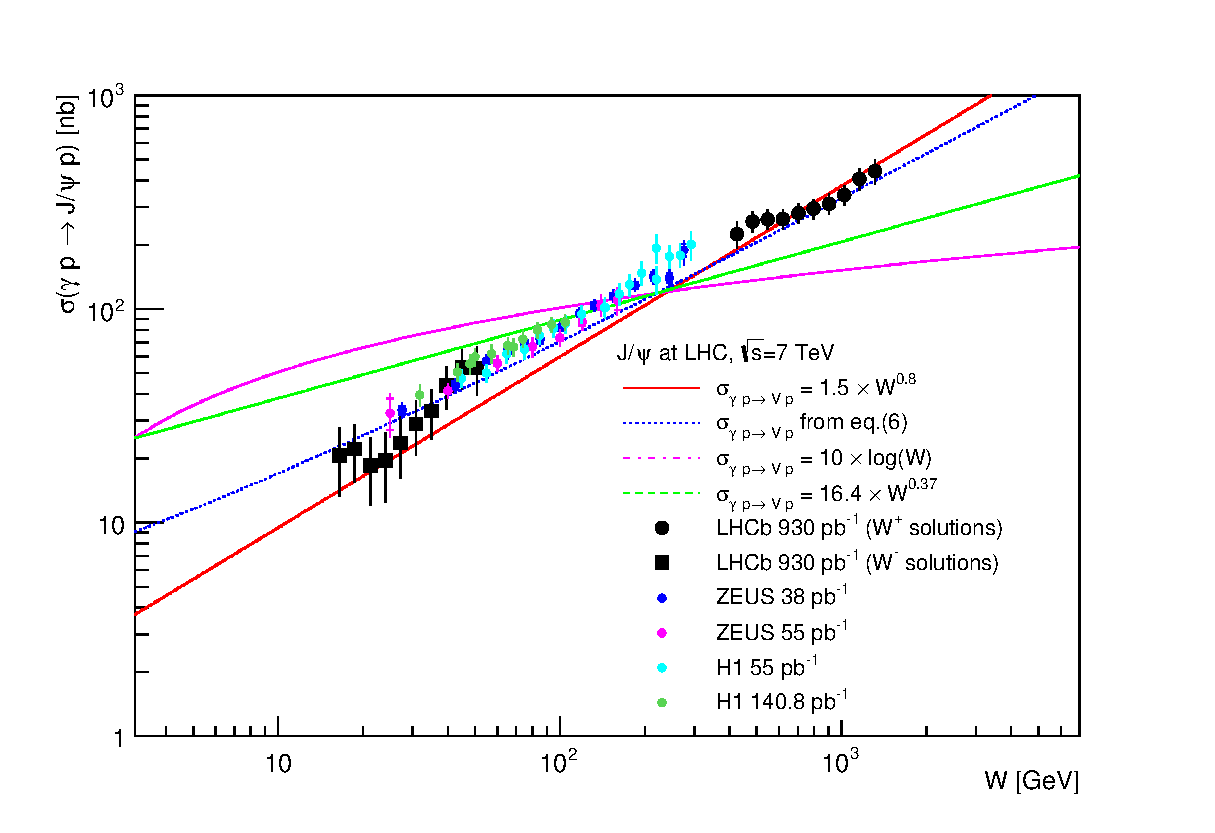
\includegraphics[width=.8\textwidth]{figures/sigma_gamma_p_W_all_theory.eps}
 \caption{$J/\psi$ photoproduction ($\gamma p \to J/\psi p$) cross section as a function photon-proton centre-of-mass energy compared
           with LHCb, ZEUS and H1 data. Other details are as in Figure~\ref{fig:all_curves}.}
 \label{fig:all_curves_w}
\end{figure}

\section{Conclusions and Outlook}

In this work, predictions for exclusive $J/\Psi$ meson production at the LHC were presented and compared to recent data from LHCb.
Predictions for HERA were also shown and compared to H1 and ZEUS data.
The simple power-law and a more advanced geometric model were used to describe the photon-proton cross section.
The rapidity data from LHCb are steeper than predictions. A better description can be obtained by tuning the power,
however this makes the predictions inconsistent with HERA. 

This is only a first look which we plan to extend in the following ways:
\begin{itemize}
\item Inclusion of $t$ dependence - both exponential (corresponding to linear Regge trajectories) and with deviations from the exponential (from linar Regge trajectories);
\item Dependence of the $\sigma_{\gamma p \rightarrow V p}$ cross section on $Q^2$, negligible in $\gamma-$ but important in Reggeon (Pomeron, Odderon,...) exchanges.
\item Study of inelastic processes, that is when additional particles are produced due to either gluon radiation and/or (c,d) proton dissociation;
\item More advanced studies of corrections due to rapidity gap survival probability.
\end{itemize}

% A more advanced version of the Reggeometric model, Ref. \cite{Fazio}b) includes also $Q^2-$ dependence (electroproduction), the universal "Reggeometric" Pomeron containing two terms, a "hard" and a "soft" one, their relative weight depending on $\tilde Q^2$. Te relevant scattering amplitude is quoted in Eq. (13) of Ref. \cite{Fazio}b) with the fitted parameters collected in Tables 2 to 4 of of the same paper.

% \section*{Acknowledgements}

\begin{thebibliography}{99}
\bibitem{LHCb1} LHCb Collab., R. Aaji {\it et al., Exclusive ...}, J. Phys. {\bf G40} (2013) 045001, arXiv:1301.7084.

\bibitem{LHCb2}  LHCb Collab., R. Aaji {\it et al., Updated ...}, arXiv:1401.3288.

\bibitem{Schafer} A. Sch\"afer, L. Mankiewicz and O. Nachtmann, Phys. Lett. {\bf B272} (1991) 419.

\bibitem{Review} G. Baur {\it et al.} Phys. Rept. {\bf 364} (2002) 359, arXiv: hep-ph/011221; K. Hencken {\it et al.}, in: Phys. Rept. {\bf 458} (2008) 1.

\bibitem{Brazil} a) V.P. Goncalves and M.M. Machado, {\it Heavy quark production...}, arXiv: 1112.3500;
b) V.P. Goncalves and M.M. Machado, {\it Quarkonium+...}, arXiv: 1207.5273 [hep-ph]; c) V.P. Gonsalves and W.K. Suter, arXiv: 1004.1952 [hep-ph];
d) V.P. Goncalves and M.M. Machado, {\it Vector meson production...}, arXiv: 1106.3036 [hep-ph]; e) V.P. Goncalves, {\it Probing the Odderon...},
arXiv: 1211.1207 [hep-ph]; f) M.B. Gay Ducati, M.T. Griep and M.V.T. Machado, {\it Exclusive photoproduction of...}, arXiv: 1305.4611 [hep-ph];
g) V.P. Goncalves and M.M. Machado, {\it Photoproduction of ...}, arXiv: 0907.4123 [hep-ph].

\bibitem{FFJS} a) S. Fazio, R. Fiore, L. Jenkovszky, A. Salii, Acta Phys. Polonica B {\bf 44} (2013) N6, 1333; b) S. Fazio, R. Fiore, L. Jenkovszky, A. Salii,
hep-ph/1312.5683, Dec. 2013, Phys. Rev. D, to be published. 


\bibitem{Ryskin} a) V.A. Khoze, A.D. Martin, and M.G. Ryskin, {\it Photon-exchange...}, arXiv: 0201301 [hep-ph];
b) S.P. Jones, A.D. Martin, and M.G. Ryskin and T. Teubner, {\it Probes of...} arXiv:1307.7099 [hep-ph];
c) S.P. Jones, A.D. Martin, and M.G. Ryskin and T. Teubner, {\it Predictions of...} arXiv: 1312.6795 [hep-ph].

\bibitem{Motyka} a) A. Bzdak {\it et al., Exclusive...}, arXive:hep/ph/0702134; b) L. Motyka and G. Watt, {\it Exclusive...}, arXiv:0805.2113.

\bibitem{Szczurek} a) W. Sch\"afer and A. Szczurek, {\it Exclusive...}, arXiv:0705.2887 [hep-ph]; b) W. Sch\"afer, G. Slipek and A. Szczurek,
{\it Exclusive...} Phys. Letters {\bf B688} (2010) 185.

\bibitem{Recent} arXiv'es: 1404.0896, 1405.2112, 1405.2112,...?

\bibitem{DL} A. Donnachie and P. Landshoff, Phys. Lett. {\bf B296} (1992) 227.

\bibitem{Francesco} R. Fiore, L.L. Jenkovszky, F. Paccanoni, EPJ {\bf C10} (1999) 461; arXiv hep-ph/9812458.

\bibitem{Capua} M. Capua {\it et al.}, Phys, Lett. {B645} (1997) 161; hep-ph/0605319


\end{thebibliography}

\end{document}
